% ============================================================
%  MEMRES — FSE-AIWare 2026  |  Slide Deck
%  Style: Madrid (stripped) + Navy/White/Gold palette
%         + TikZ overlay title/thankyou + pgfplots + fontawesome
% ============================================================
\documentclass[aspectratio=169]{beamer}
\usetheme{Madrid}

% --- Packages ---
\usepackage[utf8]{inputenc}
\usepackage[T1]{fontenc}
\usepackage{graphicx}
\usepackage{booktabs}
\usepackage{xcolor}
\usepackage{tikz}
\usetikzlibrary{shapes.geometric, arrows.meta, positioning, calc,
  patterns, decorations.pathreplacing, fit, backgrounds}
\usepackage{pgfplots}
\pgfplotsset{compat=1.18}
\usepackage{fontawesome5}
\usepackage{array}
\usepackage{colortbl}

% ==============================
%  COLOR PALETTE  (corporate / academic modern)
% ==============================
\definecolor{navydark}{RGB}{10,25,49}
\definecolor{navymid}{RGB}{22,48,85}
\definecolor{navylight}{RGB}{42,75,120}
\definecolor{warnorange}{RGB}{235,137,33}
\definecolor{successgreen}{RGB}{46,174,86}
\definecolor{goldaccent}{RGB}{255,193,7}
\definecolor{lightgray}{RGB}{240,243,247}
\definecolor{softwhite}{RGB}{248,249,252}

% Override beamer colors
\setbeamercolor{palette primary}{bg=navydark,fg=white}
\setbeamercolor{palette secondary}{bg=navymid,fg=white}
\setbeamercolor{palette tertiary}{bg=navydark,fg=white}
\setbeamercolor{palette quaternary}{bg=navydark,fg=white}
\setbeamercolor{structure}{fg=navydark}
\setbeamercolor{title}{fg=white,bg=navydark}
\setbeamercolor{frametitle}{fg=white,bg=navydark}
\setbeamercolor{block title}{bg=navymid,fg=white}
\setbeamercolor{block body}{bg=lightgray,fg=black}
\setbeamercolor{block title alerted}{bg=warnorange,fg=white}
\setbeamercolor{block body alerted}{bg=warnorange!8,fg=black}
\setbeamercolor{block title example}{bg=successgreen,fg=white}
\setbeamercolor{block body example}{bg=successgreen!8,fg=black}
\setbeamercolor{item}{fg=navymid}
\setbeamercolor{subitem}{fg=navylight}
\setbeamercolor{enumerate item}{fg=navydark}
\setbeamercolor{section in toc}{fg=navydark}
\setbeamercolor{footline}{bg=navydark,fg=white}

\setbeamerfont{frametitle}{series=\bfseries}

% Pre-define TikZ styles with parameters (must be in preamble for beamer)
\tikzset{
  pipestage/.style={draw=navydark, very thick, rounded corners=5pt,
    minimum height=1cm, minimum width=2.6cm, align=center,
    font=\small\bfseries, text=white},
  pipesub/.style={draw=#1!70, thick, rounded corners=3pt,
    fill=#1!12, minimum height=0.55cm, minimum width=1.6cm,
    align=center, font=\scriptsize, text=#1!80!black},
  pipestore/.style={draw=#1, very thick, rounded corners=6pt,
    fill=#1!10, minimum height=0.65cm, align=center,
    font=\scriptsize\bfseries, text=#1!80!black},
}

% Short author / institute for footer
\title[MEMRES]{MEMRES}
\subtitle{Memory-Augmented Agentic Python Dependency Resolver}
\author[Tran et al.]{%
  Chi-Nguyen Tran \and Sy-Duy-Minh Dao \and Trung-Kiet Huynh \and
  Phu-Hoa Pham \and Lam-Phu-Quy Nguyen}
\institute[VNU-HCM]{University of Science, VNU-HCM}
\date{FSE-AIWare 2026}

% ============================================================
\begin{document}

% ==================  TITLE SLIDE  ===========================
{%
\setbeamertemplate{footline}{}
\begin{frame}[plain]
\begin{tikzpicture}[remember picture,overlay]

  %--- Background layers with depth ----
  \fill[navydark]
    (current page.south west) rectangle (current page.north east);
  \fill[navymid, opacity=0.55]
    ([yshift=1.2cm]current page.south west) rectangle
    ([yshift=-0.5cm]current page.north east);
  \fill[navylight, opacity=0.25]
    ([yshift=3cm]current page.south west) rectangle
    ([yshift=-1.8cm]current page.north east);

  %--- Orange separator ---
  \draw[warnorange, line width=2.5pt]
    ([yshift=-2.3cm,xshift=2cm]current page.north west) --
    ([yshift=-2.3cm,xshift=-2cm]current page.north east);

  %--- Title text ---
  \node[anchor=south, text=white, font=\Huge\bfseries]
    at ([yshift=0.6cm]current page.center) {MEMRES};

  \node[anchor=north, text=white!85, font=\large, text width=12cm, align=center]
    at ([yshift=0.4cm]current page.center)
    {Memory-Augmented Agentic Python Dependency Resolver};

  %--- Authors ---
  \node[anchor=north, text=white!70, font=\small, text width=13cm, align=center]
    at ([yshift=-0.7cm]current page.center)
    {Chi-Nguyen Tran\quad$\cdot$\quad Sy-Duy-Minh Dao\quad$\cdot$\quad Trung-Kiet Huynh\quad$\cdot$\quad Phu-Hoa Pham\quad$\cdot$\quad Lam-Phu-Quy Nguyen\\[3pt]
     {\scriptsize \{23122044, 23122041, 23122039, 23122030, 23122048\}@student.hcmus.edu.vn}};

  %--- Institute ---
  \node[anchor=north, text=white!55, font=\footnotesize]
    at ([yshift=-1.6cm]current page.center)
    {University of Science, VNU-HCM};

  %--- Result badge ---
  \node[fill=successgreen, rounded corners=6pt, inner sep=6pt,
        font=\normalsize\bfseries, text=white]
    at ([yshift=-2.5cm]current page.center)
    {\faCheckCircle\quad 87.2\% Success on HG2.9K};

  %--- Conference ---
  \node[anchor=south, text=white!40, font=\scriptsize]
    at ([yshift=0.4cm]current page.south)
    {FSE-AIWare 2026\quad$\cdot$\quad Montreal, Canada\quad$\cdot$\quad July 5--9, 2026};

\end{tikzpicture}
\end{frame}
}

% ==================  MOTIVATION  ============================
\begin{frame}{Motivation}
\begin{columns}[T]

\begin{column}{0.55\textwidth}
\begin{block}{\faExclamationTriangle\quad The Problem}
\begin{itemize}
  \item Python has \textbf{500\,000+} PyPI packages ---\\
        dependency conflicts are \emph{pervasive}.
  \item Legacy snippets frequently fail with\\
        \texttt{ImportError}, \texttt{SyntaxError}, version mismatch.
\end{itemize}
\end{block}

\begin{alertblock}{\faBug\quad PLLM Baseline}
\begin{itemize}
  \item Only \textbf{54.7\%} success rate on HG2.9K.
  \item 1\,308 snippets remain \emph{unresolved}.
\end{itemize}
\end{alertblock}

\begin{exampleblock}{\faLightbulb[regular]\quad Our Solution}
An \textbf{agentic, memory-augmented} approach that minimizes LLM reliance via a confidence cascade.
\end{exampleblock}
\end{column}

\begin{column}{0.42\textwidth}
\centering
\begin{tikzpicture}[scale=0.72, every node/.style={font=\scriptsize}]
  \node[draw=navymid, thick, rounded corners=4pt, fill=navymid!10,
        minimum width=3cm, minimum height=0.7cm, align=center,
        font=\scriptsize\bfseries, text=navydark]
    (snippet) at (0,3.2) {\faPython\  Python Snippet};
  \node[draw=navylight, thick, rounded corners=4pt, fill=navylight!10,
        minimum width=3cm, minimum height=0.7cm, align=center]
    (imp) at (0,1.9) {\texttt{import X, Y, Z}};
  \node[draw=red!60, thick, rounded corners=3pt, fill=red!8,
        minimum width=2.1cm, minimum height=0.6cm, align=center]
    (err1) at (-1.8,0.3) {\faTimesCircle\ ImportError};
  \node[draw=red!60, thick, rounded corners=3pt, fill=red!8,
        minimum width=2.1cm, minimum height=0.6cm, align=center]
    (err2) at (1.8,0.3) {\faTimesCircle\ SyntaxError};
  \node[draw=warnorange, thick, rounded corners=3pt, fill=warnorange!10,
        minimum width=2.5cm, minimum height=0.6cm, align=center]
    (err3) at (0,-0.9) {\faExclamationTriangle\ VersionConflict};
  \draw[-{Stealth}, thick, navymid] (snippet) -- (imp);
  \draw[-{Stealth}, thick, red!70] (imp) -- (err1);
  \draw[-{Stealth}, thick, red!70] (imp) -- (err2);
  \draw[-{Stealth}, thick, warnorange] (imp) -- (err3);
  \node[fill=red!15, rounded corners=3pt, inner sep=3pt,
        font=\scriptsize\bfseries, text=red!70]
    at (0,-1.9) {45.3\% unresolved (PLLM)};
\end{tikzpicture}
\end{column}

\end{columns}
\end{frame}

% ==================  COMPETITION  ===========================
\begin{frame}{FSE-AIWare 2026 Competition}
\begin{center}
\begin{tikzpicture}[
  scale=0.85,
  every node/.style={font=\small},
  infobox/.style={draw=navymid, thick, rounded corners=5pt,
    fill=navymid!6, minimum width=3.4cm, minimum height=1cm,
    align=center, text=navydark}
]
  % Central hub
  \node[draw=navydark, very thick, rounded corners=10pt,
        fill=navydark, text=white,
        minimum width=4.5cm, minimum height=1.2cm,
        align=center, font=\normalsize\bfseries]
    (hub) at (0,0) {\faTrophy\ FSE-AIWare 2026\\Tool Competition};

  \node[infobox] (task) at (-5, 1.8)
    {\faCode\ \textbf{Task}\\Python Dep.\ Resolution};
  \node[infobox] (data) at (5, 1.8)
    {\faDatabase\ \textbf{Dataset}\\HG2.9K (2\,890 snippets)};
  \node[infobox] (cons) at (-5, -1.8)
    {\faServer\ \textbf{Constraints}\\Docker, 10\,GB VRAM};
  \node[infobox] (met) at (5, -1.8)
    {\faChartBar\ \textbf{Metrics}\\Success, Speed, Cost};

  \draw[-{Stealth}, thick, navylight] (task) -- (hub);
  \draw[-{Stealth}, thick, navylight] (data) -- (hub);
  \draw[-{Stealth}, thick, navylight] (cons) -- (hub);
  \draw[-{Stealth}, thick, navylight] (met)  -- (hub);

  \node[font=\footnotesize, text=navylight]
    at (0, -3.3) {Montreal, Canada\quad$\cdot$\quad July 5--9, 2026\quad$\cdot$\quad ACM Digital Library};
\end{tikzpicture}
\end{center}
\end{frame}

% ==================  PIPELINE  ==============================
\begin{frame}{MEMRES System Architecture}

\begin{center}
\begin{tikzpicture}[
  scale=0.62, transform shape,
  node distance=0.4cm and 0.9cm,
  >=Stealth,
  every node/.style={font=\small},
  arrow/.style={->, very thick, navymid},
  dasharr/.style={->, thick, dashed},
]

  % --- INPUT ---
  \node[draw=navylight, very thick, rounded corners=5pt,
        fill=navylight!10, minimum height=0.9cm, minimum width=2.4cm,
        font=\small\bfseries, text=navydark] (inp) {\faPython\ Snippet};

  % --- STAGE 1 ---
  \node[pipestage, fill=navymid, right=1.4cm of inp] (s1)
    {\faMemory\ Stage 1\\Session\\Memory};

  % --- STAGE 2 ---
  \node[pipestage, fill=navylight, right=1.4cm of s1] (s2)
    {\faSearch\ Stage 2\\Hybrid\\Evaluation};
  \node[pipesub=navylight, above=0.4cm of s2, xshift=-0.9cm] (py2)
    {\scriptsize \faPython\ Py2};
  \node[pipesub=navylight, above=0.4cm of s2, xshift=0.9cm] (sem)
    {\scriptsize \faProjectDiagram\ Semantic};

  % --- STAGE 3 ---
  \node[pipestage, fill=warnorange!85!black, right=1.4cm of s2] (s3)
    {\faLayerGroup\ Stage 3\\Version\\Selection};
  \node[pipesub=warnorange, above=0.55cm of s3, xshift=-0.7cm, minimum width=1.1cm]
    (det) {\scriptsize \faCogs\ L1--L5};
  \node[pipesub=red, above=0.55cm of s3, xshift=0.7cm, minimum width=1.1cm]
    (llm) {\scriptsize \faRobot\ L6};

  % --- STAGE 4 ---
  \node[pipestage, fill=red!55!navydark, right=1.4cm of s3] (s4)
    {\faServer\ Stage 4\\Build Loop\\+ Reflexion};
  \node[pipesub=red, above=0.4cm of s4, xshift=-0.9cm] (dock)
    {\scriptsize \faDocker\ Docker};
  \node[pipesub=red, above=0.4cm of s4, xshift=0.9cm] (sys)
    {\scriptsize \faCog\ Sys-Dep};

  % --- OUTPUT ---
  \node[fill=successgreen, rounded corners=5pt, very thick,
        draw=successgreen!70!black,
        minimum height=0.7cm, minimum width=1.6cm,
        font=\small\bfseries, text=white,
        right=1.4cm of s4, yshift=0.35cm] (ok) {\faCheckCircle\ Pass};
  \node[fill=red!65, rounded corners=5pt, very thick,
        draw=red!50!black,
        minimum height=0.7cm, minimum width=1.6cm,
        font=\small\bfseries, text=white,
        right=1.4cm of s4, yshift=-0.35cm] (fail) {\faTimesCircle\ Fail};

  % === MAIN FLOW ===
  \draw[arrow] (inp) -- (s1);
  \draw[arrow] (s1) -- (s2);
  \draw[arrow] (s2) -- (s3);
  \draw[arrow] (s3) -- (s4);
  \draw[arrow] (s4) -- (ok);
  \draw[arrow] (s4) -- (fail);

  % === FAST PATH 1: cache hit (topmost line) ===
  \draw[->, very thick, successgreen!80!black, rounded corners=6pt]
    (s1.north) -- ++(0,3.2)
    node[above right=-1pt and 2pt, font=\tiny\bfseries, text=successgreen!70!black]
      {\faForward\ cache hit}
    -| (ok.north);

  % === FAST PATH 2: Py2 fast (lower line) ===
  \draw[->, very thick, successgreen!55!black, rounded corners=6pt]
    (py2.north) -- ++(0,1.6)
    node[above right=-1pt and 2pt, font=\tiny\bfseries, text=successgreen!55!black]
      {\faForward\ Py2 fast}
    -| ([xshift=-0.15cm]ok.north);

  % === RETRY ===
  \draw[dasharr, warnorange, very thick, rounded corners=4pt]
    (s4.south) -- ++(0,-0.7) -| (s3.south)
    node[midway, below, font=\tiny\bfseries, text=warnorange]
    {\faRedo\ retry ($\leq$10$\times$)};

  % === CASCADE BRACE (drawn before memory/KB so brace is on top) ===
  \draw[decorate, decoration={brace, amplitude=4pt, mirror}, very thick, navydark]
    ([yshift=-1.1cm]s2.south west) -- ([yshift=-1.1cm]s3.south east)
    node[midway, below=6pt, font=\tiny\bfseries, text=navydark]
    {Confidence Cascade};

  % === MEMORY ===
  \node[pipestore=purple, below=2.8cm of s2, minimum width=3.4cm]
    (memory) {\faBrain\ Self-Evolving Memory\\[-1pt]{\tiny Tips + Shortcuts (Jaccard $\geq$0.5)}};
  \draw[dasharr, purple!60] (memory.north) -- (s2.south)
    node[midway, right, font=\tiny, text=purple!60] {read};
  \draw[dasharr, purple!60] (s4.south) |- ([yshift=0.15cm]memory.east)
    node[near end, above, font=\tiny, text=purple!60] {write};
  \draw[dasharr, purple!60] (memory.west) -| ([xshift=0.2cm]s1.south)
    node[near start, below, font=\tiny, text=purple!60] {lookup};

  % === KB ===
  \node[pipestore=warnorange!80!black, below=2.8cm of s3, minimum width=3cm]
    (kb) {\faBook\ Error Pattern KB\\[-1pt]{\tiny 200+ mappings, 35 corrections}};
  \draw[dasharr, warnorange!70] (kb.north) -- (s3.south)
    node[midway, right, font=\tiny, text=warnorange!70] {query};
  \draw[dasharr, warnorange!70] (s4.south east) |- ([yshift=-0.15cm]kb.east)
    node[near end, below, font=\tiny, text=warnorange!70] {learn};

\end{tikzpicture}
\end{center}

\vspace{-0.4em}
\begin{columns}[T]
\begin{column}{0.48\textwidth}
\begin{itemize}\small
  \item[\faLayerGroup] Multi-level confidence cascade
  \item[\faBrain] Memory-augmented: reuse proven solutions
\end{itemize}
\end{column}
\begin{column}{0.48\textwidth}
\begin{itemize}\small
  \item[\faBook] Error Pattern KB: 200+ mappings
  \item[\faPython] Py2 detector, sys-dep injection
\end{itemize}
\end{column}
\end{columns}
\end{frame}

% ==================  CONFIDENCE CASCADE  ====================
\begin{frame}{Confidence Cascade}
\begin{center}
\begin{tikzpicture}[
  scale=0.75, transform shape,
  every node/.style={font=\small},
  lvl/.style={draw=navymid, thick, rounded corners=5pt,
    minimum width=4cm, minimum height=0.6cm, align=center,
    font=\small\bfseries, text=white},
]
  \node[lvl, fill=successgreen!80!black] (l1) at (0,5) {\faMemory\ L1: Session Memory};
  \node[lvl, fill=successgreen!65!black] (l2) at (0,4) {\faMap\ L2: Compatibility Map};
  \node[lvl, fill=goldaccent!80!black] (l3) at (0,3) {\faCubes\ L3: Ecosystem Templates};
  \node[lvl, fill=goldaccent!65!black] (l4) at (0,2) {\faProjectDiagram\ L4: Co-occurrence};
  \node[lvl, fill=warnorange!85!black] (l5) at (0,1) {\faCogs\ L5: Heuristic Rules};
  \node[lvl, fill=red!65!black] (l6) at (0,0) {\faRobot\ L6: LLM Fallback};

  % miss arrows
  \draw[-{Stealth}, thick, navylight] (l1) -- (l2) node[midway, right=3pt, font=\tiny, text=navylight] {miss};
  \draw[-{Stealth}, thick, navylight] (l2) -- (l3) node[midway, right=3pt, font=\tiny, text=navylight] {miss};
  \draw[-{Stealth}, thick, navylight] (l3) -- (l4) node[midway, right=3pt, font=\tiny, text=navylight] {miss};
  \draw[-{Stealth}, thick, navylight] (l4) -- (l5) node[midway, right=3pt, font=\tiny, text=navylight] {miss};
  \draw[-{Stealth}, thick, navylight] (l5) -- (l6) node[midway, right=3pt, font=\tiny, text=navylight] {miss};

  % Resolved badge
  \node[fill=successgreen, rounded corners=6pt, inner sep=6pt,
        font=\small\bfseries, text=white] (res) at (5.5, 2.5)
    {\faCheckCircle\ Resolved!};

  \draw[-{Stealth}, dashed, successgreen!60, thick] (l1.east) -- ++(0.5,0) |- (res);
  \draw[-{Stealth}, dashed, successgreen!60, thick] (l2.east) -- ++(0.5,0) |- (res);
  \draw[-{Stealth}, dashed, successgreen!60, thick] (l3.east) -- ++(0.5,0) |- (res);
  \draw[-{Stealth}, dashed, successgreen!60, thick] (l4.east) -- ++(0.5,0) |- (res);
  \draw[-{Stealth}, dashed, successgreen!60, thick] (l5.east) -- ++(0.5,0) |- (res);
  \draw[-{Stealth}, dashed, successgreen!60, thick] (l6.east) -- ++(0.5,0) |- (res);

  % Labels
  \node[font=\scriptsize, text=successgreen!70!black, anchor=east] at (-2.8,5) {Deterministic};
  \node[font=\scriptsize, text=successgreen!70!black, anchor=east] at (-2.8,4) {Deterministic};
  \node[font=\scriptsize, text=goldaccent!70!black, anchor=east]  at (-2.8,3) {Deterministic};
  \node[font=\scriptsize, text=goldaccent!70!black, anchor=east]  at (-2.8,2) {Deterministic};
  \node[font=\scriptsize, text=warnorange!70!black, anchor=east]  at (-2.8,1) {Deterministic};
  \node[font=\scriptsize, text=red!70!black, anchor=east]         at (-2.8,0) {LLM-based};

  % Brace
  \draw[decorate, decoration={brace, amplitude=5pt}, very thick, navydark]
    (-2.6,5.35) -- (-2.6,1.35)
    node[midway, left=8pt, font=\scriptsize\bfseries, text=navydark, rotate=90, anchor=south]
    {No LLM needed};

  \node[fill=navydark!8, rounded corners=4pt, inner sep=5pt,
        font=\small, text=navydark] at (1.5,-1.3)
    {First hit terminates cascade\quad$\cdot$\quad \textbf{60\%+} fewer LLM calls};

\end{tikzpicture}
\end{center}
\end{frame}

% ==================  KEY TECHNIQUES  ========================
\begin{frame}{Key Techniques}
\begin{columns}[T]

\begin{column}{0.48\textwidth}
\begin{block}{\faMemory\quad Memory Systems}
\begin{itemize}\small
  \item \textbf{Intra-Session Memory}:\\
        Cache successful solutions for similar snippets.
  \item \textbf{Self-Evolving Memory}:\\
        Learn tips/shortcuts via Jaccard similarity.
\end{itemize}
\end{block}

\begin{block}{\faCogs\quad Analysis}
\begin{itemize}\small
  \item \textbf{Semantic Analyzer}:\\
        Import usage patterns, ecosystem detection.
  \item \textbf{Python 2 Detector}:\\
        13 indicators, auto interpreter selection.
\end{itemize}
\end{block}
\end{column}

\begin{column}{0.48\textwidth}
\begin{block}{\faBook\quad Knowledge Base}
\begin{itemize}\small
  \item \textbf{Error Pattern KB}:\\
        200+ mappings, name corrections,\\
        version constraints, regex rules.
\end{itemize}
\end{block}

\begin{block}{\faServer\quad Build \& Deploy}
\begin{itemize}\small
  \item \textbf{System Dependency Injection}:\\
        \texttt{apt-get} for C-extensions,\\
        version fallback cascade.
  \item \textbf{Reflexion Loop}:\\
        Up to 10 retries with error-guided repair.
\end{itemize}
\end{block}
\end{column}

\end{columns}
\end{frame}

% ==================  EVALUATION  ============================
\begin{frame}{Evaluation: MEMRES vs.\ PLLM}
\begin{columns}[T]

\begin{column}{0.45\textwidth}
\centering
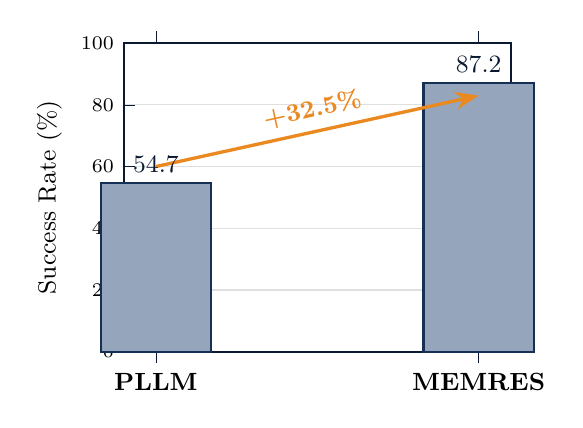
\begin{tikzpicture}
\begin{axis}[
  ybar,
  width=6.5cm, height=5.5cm,
  bar width=1.4cm,
  ymin=0, ymax=100,
  ylabel={\small Success Rate (\%)},
  ylabel style={font=\small},
  symbolic x coords={PLLM, MEMRES},
  xtick=data,
  xticklabel style={font=\small\bfseries},
  ytick={0,20,40,60,80,100},
  yticklabel style={font=\scriptsize},
  ymajorgrids=true,
  grid style={gray!25},
  axis line style={thick, navydark},
  tick style={navydark},
  nodes near coords,
  every node near coord/.append style={font=\small\bfseries, text=navydark},
  nodes near coords align={vertical},
  clip=false,
]
  \addplot[fill=navylight!50, draw=navymid, thick]
    coordinates {(PLLM, 54.7) (MEMRES, 87.2)};

  % Delta annotation
  \draw[-{Stealth}, very thick, warnorange]
    (axis cs:PLLM, 60) -- (axis cs:MEMRES, 83)
    node[midway, above, sloped, font=\small\bfseries, text=warnorange]
    {+32.5\%};
\end{axis}
\end{tikzpicture}
\end{column}

\begin{column}{0.52\textwidth}
\small
\begin{tabular}{l r r}
  \toprule
  \textbf{Metric} & \textbf{PLLM} & \textbf{MEMRES} \\
  \midrule
  Resolved  & 1\,583 & \cellcolor{successgreen!15}\textbf{2\,519} \\
  Failed    & 1\,308 & \cellcolor{successgreen!15}\textbf{371} \\
  Success   & 54.7\% & \cellcolor{successgreen!15}\textbf{87.2\%} \\
  \bottomrule
\end{tabular}

\vspace{0.6em}
\begin{exampleblock}{\faCheckCircle\quad Key Results}
\begin{itemize}\small
  \item Setup: HG2.9K, Gemma-2 9B, Docker
  \item \textbf{950+} PLLM failures resolved
  \item 53.9\% needed sys-dep classifiers
\end{itemize}
\end{exampleblock}
\end{column}

\end{columns}
\end{frame}

% ==================  ABLATION  ==============================
\begin{frame}{Ablation Study: Resolution by Component}
\begin{center}
\begin{tikzpicture}
\begin{axis}[
  xbar stacked,
  width=13cm, height=3cm,
  xmin=0, xmax=100,
  xlabel={\small Resolved Snippets (\%)},
  xlabel style={font=\small},
  ytick=\empty,
  xtick={0,20,40,60,80,100},
  xticklabel style={font=\scriptsize},
  xmajorgrids=true,
  grid style={gray!20},
  axis line style={thick, navydark},
  legend style={at={(0.5,-0.55)}, anchor=north, legend columns=4,
    font=\scriptsize, draw=none, fill=none},
  bar width=1cm,
  clip=false,
]
  \addplot[fill=successgreen!55, draw=successgreen!70!black, thick]
    coordinates {(41.8, 0)};
  \addplot[fill=goldaccent!60, draw=goldaccent!70!black, thick]
    coordinates {(16.1, 0)};
  \addplot[fill=warnorange!50, draw=warnorange!70!black, thick]
    coordinates {(10.2, 0)};
  \addplot[fill=red!40, draw=red!60!black, thick]
    coordinates {(31.9, 0)};

  \legend{Session Memory (41.8\%), Py2 Heuristic (16.1\%), Deterministic L2--5 (10.2\%), LLM Fallback (31.9\%)}
\end{axis}

% Deterministic brace
\draw[decorate, decoration={brace, amplitude=5pt, mirror}, very thick, navydark]
  (0,-0.6) -- (8.8,-0.6)
  node[midway, below=7pt, font=\small\bfseries, text=navydark]
  {\faLock\ 68\% Deterministic (No LLM)};

% Total label
\node[fill=navydark!8, rounded corners=4pt, inner sep=4pt,
      font=\small\bfseries, text=navydark] at (6.5,2.2)
  {Total: 2\,519 resolved (100\%)};

\end{tikzpicture}
\end{center}

\vspace{0.2em}
\begin{columns}[T]
\begin{column}{0.32\textwidth}
\begin{exampleblock}{\faCheckCircle\ Memory}
\small 41.8\% via cached solutions --- zero LLM cost.
\end{exampleblock}
\end{column}
\begin{column}{0.32\textwidth}
\begin{block}{\faPython\ Python 2}
\small Resolves the single largest PLLM failure category.
\end{block}
\end{column}
\begin{column}{0.32\textwidth}
\begin{alertblock}{\faRobot\ LLM}
\small Only 32\% need the LLM as last resort.
\end{alertblock}
\end{column}
\end{columns}
\end{frame}

% ==================  FAILURE ANALYSIS  ======================
\begin{frame}{Failure Analysis (371 failures)}
\begin{center}
\small
\begin{tabular}{>{\raggedright}p{2.8cm} l r r}
  \toprule
  \textbf{Category} & \textbf{Root Cause} & \textbf{Count} & \textbf{\%} \\
  \midrule
  \rowcolor{red!8}
  \faWrench\ Build / C-ext    & Missing C toolchains      & 186 & 50.1\% \\
  \rowcolor{warnorange!8}
  \faBoxOpen\ ImportError      & Obscure/deprecated pkgs   & 121 & 32.6\% \\
  \rowcolor{goldaccent!10}
  \faClock\ Timeout            & Large ML compilation      &  55 & 14.8\% \\
  \faDesktop\ System/Platform  & GTK, RPi, platform-only   &   9 &  2.4\% \\
  \midrule
  \textbf{Total}               &                           & \textbf{371} & \textbf{100\%} \\
  \bottomrule
\end{tabular}
\end{center}

\vspace{0.3em}
\begin{columns}[T]
\begin{column}{0.48\textwidth}
\begin{alertblock}{\faExclamationTriangle\quad Inherent Limits}
\small
Most failures are \textbf{inherently unresolvable} in Docker --- no C toolchain, no GPU.
\end{alertblock}
\end{column}
\begin{column}{0.48\textwidth}
\begin{block}{\faInfoCircle\quad Insight}
\small
32.6\% from packages completely absent from PyPI (deprecated/renamed). Only 2.4\% platform-specific.
\end{block}
\end{column}
\end{columns}
\end{frame}

% ==================  LIMITATIONS  ===========================
\begin{frame}{Limitations \& Lessons Learned}
\begin{columns}[T]

\begin{column}{0.48\textwidth}
\begin{alertblock}{\faExclamationCircle\quad Limitations}
\begin{itemize}\small
  \item C-extension build errors dominate failures.
  \item Session memory is \emph{order-sensitive}.
  \item Runtime passes (system-only imports) are\\
        strictly counted as failures.
\end{itemize}
\end{alertblock}
\end{column}

\begin{column}{0.48\textwidth}
\begin{exampleblock}{\faGraduationCap\quad Lessons}
\begin{itemize}\small
  \item Deterministic rules + memory outperform LLM-only.
  \item Error KB dramatically reduces repeat failures.
  \item Batch ordering affects memory effectiveness.
\end{itemize}
\end{exampleblock}
\end{column}

\end{columns}

\vspace{0.8em}
\begin{center}

\begin{tikzpicture}
  \node[fill=navydark!8, rounded corners=5pt, inner sep=8pt,
        font=\small, text=navydark, text width=10cm, align=center]
  {\faQuoteLeft\quad \emph{``The best LLM call is the one you never make.''}
   \quad\faQuoteRight\\[3pt]
   \textbf{--- Key design principle of MEMRES}};
\end{tikzpicture}
\end{center}
\end{frame}

% ==================  CONCLUSION  ============================
\begin{frame}{Conclusion}
\begin{block}{\faFlag\quad Summary}
\begin{itemize}
  \item MEMRES: agentic resolver with \textbf{memory augmentation} and \textbf{confidence cascade}.
  \item Achieves \textbf{87.2\%} success on HG2.9K, surpassing PLLM (54.7\%) by \textbf{+32.5\%}.
  \item Reduces LLM calls by \textbf{60\%+} via deterministic-first design.
\end{itemize}
\end{block}

\vspace{0.4em}
\begin{exampleblock}{\faStar\quad Contributions}
\begin{itemize}
  \item Novel 4-stage pipeline with multi-level confidence cascade.
  \item Error Pattern KB (200+ mappings) + Self-Evolving Memory.
  \item Python 2 heuristics + System dependency injection.
\end{itemize}
\end{exampleblock}

\vspace{0.4em}
\begin{center}

\begin{tikzpicture}
  \node[fill=successgreen, rounded corners=6pt, inner sep=7pt,
        font=\normalsize\bfseries, text=white]
  {\faCheckCircle\quad 2\,519 / 2\,890 snippets resolved (87.2\%)};
\end{tikzpicture}
\end{center}
\end{frame}

% ==================  THANK YOU  =============================
{%
\setbeamertemplate{footline}{}
\begin{frame}[plain]
\begin{tikzpicture}[remember picture,overlay]

  %--- Background layers ---
  \fill[navydark]
    (current page.south west) rectangle (current page.north east);
  \fill[navymid, opacity=0.5]
    ([yshift=2cm]current page.south west) rectangle
    ([yshift=-1cm]current page.north east);
  \fill[navylight, opacity=0.2]
    ([yshift=4cm]current page.south west) rectangle
    ([yshift=-2.5cm]current page.north east);

  %--- Orange separator ---
  \draw[warnorange, line width=2.5pt]
    ([yshift=1.5cm,xshift=3cm]current page.west) --
    ([yshift=1.5cm,xshift=-3cm]current page.east);

  %--- Thank you ---
  \node[text=white, font=\Huge\bfseries]
    at ([yshift=2.8cm]current page.center) {Thank You!};

  \node[text=white!75, font=\large]
    at ([yshift=1.9cm]current page.center)
    {Questions \& Discussion};

  %--- Result badge ---
  \node[fill=successgreen, rounded corners=6pt, inner sep=8pt,
        font=\large\bfseries, text=white]
    at (current page.center)
    {\faCheckCircle\quad 87.2\% Success Rate};

  %--- Contact info ---
  \node[text=white!60, font=\small, text width=12cm, align=center]
    at ([yshift=-1.6cm]current page.center)
    {\faEnvelope\quad \{23122044, 23122041, 23122039, 23122030, 23122048\}@student.hcmus.edu.vn};

  \node[text=white!60, font=\small]
    at ([yshift=-2.3cm]current page.center)
    {\faUniversity\quad University of Science, VNU-HCM};

  %--- GitHub ---
  \node[text=white!40, font=\footnotesize]
    at ([yshift=0.6cm]current page.south)
    {\faGithub\quad github.com/checkdgt/fse-aiware-python-dependencies};

\end{tikzpicture}
\end{frame}
}

\end{document}
